\documentclass[11pt]{article}
\usepackage[margin=1in]{geometry}
\usepackage{amsmath, amssymb}
\usepackage{tikz}
\usetikzlibrary{arrows.meta, positioning, calc}
\usepackage{hyperref}

\title{CSE 5825 --- Homework 1 Study Notes\\
\large Tools You Need, Not the Answers}
\author{}
\date{}

\begin{document}
\maketitle

These notes collect the \emph{techniques} each problem is testing. No
final numeric or symbolic answers to your specific problems are given ---
the goal is that you can produce them yourself.

\section*{Problem 1: Product Rule, Chain Rule, Bayes' Rule}

Everything here comes from one definition, applied twice:
\[
  p(u \mid v) = \frac{p(u,v)}{p(v)} \quad \Longleftrightarrow \quad p(u,v) = p(u\mid v)\,p(v).
\]

\textbf{Chain rule with an extra conditioning variable $z$.} The identity
still holds if every term is conditioned on the same extra variable $z$
throughout:
\[
  p(x,y\mid z) = p(x \mid y, z)\, p(y \mid z) = p(y \mid x,z)\, p(x\mid z).
\]
This is just the ordinary product rule applied \emph{inside} the
conditional distribution $p(\cdot \mid z)$ --- think of $p(\cdot\mid z)$
as ``a probability distribution in its own right'' and apply the same
two-variable rule you already know to it. To get the first identity
you're asked to prove, apply the product rule to $x$ and $y$ within
the world where $z$ is already given.

\textbf{Turning it into Bayes' rule.} Once you have
$p(x,y\mid z) = p(x\mid y,z)\,p(y\mid z)$, and separately
$p(x,y\mid z) = p(y \mid x, z)\, p(x \mid z)$, set the two right-hand
sides equal to each other and solve for $p(x\mid y,z)$. That produces
the second identity: a version of Bayes' rule where everything is
additionally conditioned on background information $z$. This
``conditioned throughout'' form of Bayes' rule is used constantly in
graphical models (e.g.\ conditioning on evidence you've already
observed).

\section*{Problem 2: Law of Total Probability + Bayes' Rule}

This is a two-stage random experiment: first a department is chosen,
then a student within it.

\begin{itemize}
  \item \textbf{Part (a)} is the \emph{law of total probability}: to get
        the overall probability of an event (female), sum the
        probability of that event \emph{within} each department,
        weighted by the probability of landing in that department:
        \[
          P(\text{female}) = \sum_{\text{dept}} P(\text{female}\mid \text{dept})\,P(\text{dept}).
        \]
  \item \textbf{Part (b)} is Bayes' rule run backwards: you're given the
        outcome (female) and asked about the cause (which department).
        \[
          P(\text{dept}=B \mid \text{female}) = \frac{P(\text{female}\mid \text{dept}=B)\,P(\text{dept}=B)}{P(\text{female})}.
        \]
        Note the denominator is exactly the quantity you computed in
        part (a) --- don't recompute it separately.
  \item \textbf{Part (c)} is the same idea as (b) but conditioning on
        ``male'' instead of ``female.'' You'll need
        $P(\text{male}\mid\text{dept}) = 1 - P(\text{female}\mid\text{dept})$
        and the analogous total-probability denominator for male.
\end{itemize}
A tree diagram (department branches, then male/female sub-branches with
the given percentages as edge probabilities) makes all three parts
mechanical: multiply along branches to get joint probabilities, sum
branches for totals, divide for conditionals.

\section*{Problem 3 \& 6(d): Counting Parameters of a Discrete Distribution}

\textbf{Full joint table, no structure assumed.} If variable $i$ can
take $k_i$ values, a full joint table over variables $X_1,\dots,X_m$ has
$\prod_i k_i$ entries, but the probabilities must sum to 1, so only
$\left(\prod_i k_i\right) - 1$ of them are \emph{free} (independent)
parameters --- the last one is determined by the constraint that
everything sums to 1.

\textbf{A single conditional probability table (CPT), $P(X \mid \text{Parents})$.}
If $X$ has $k$ values and its parents jointly have $r$ possible
configurations, then for \emph{each} of the $r$ parent configurations
you need a separate distribution over $X$'s $k$ values, and each of
those distributions has $k-1$ free parameters (again, one value is
determined by the sum-to-1 constraint). So a CPT costs
\[
  r \times (k - 1)
\]
free parameters, where $r$ is the product of the number of values of
each parent (or $r=1$, i.e.\ just $k-1$ parameters, if $X$ has no
parents).

\textbf{Total parameters for a factorized/network distribution.} Add up
the CPT cost (using the formula above) for every variable in the
factorization. Compare this total to the full-joint-table count from
part (a)/(b) of Problem 3 --- the gap between them is exactly what
structure (conditional independence) buys you.

\section*{Problems 3(c), 4(a), 5(a), 6(a)-(b): Reading Independence off a Graph (d-separation)}

A Bayesian network is a DAG where each node's CPT is
$P(\text{node} \mid \text{parents of node})$, and the joint is the
product of all these CPTs (this \emph{is} the factorization/chain rule
from Problem 1, applied along the graph). Whether two variables are
independent (unconditionally, or given some evidence set $Z$) is read
off the graph using three local patterns along any path between them:

\begin{center}
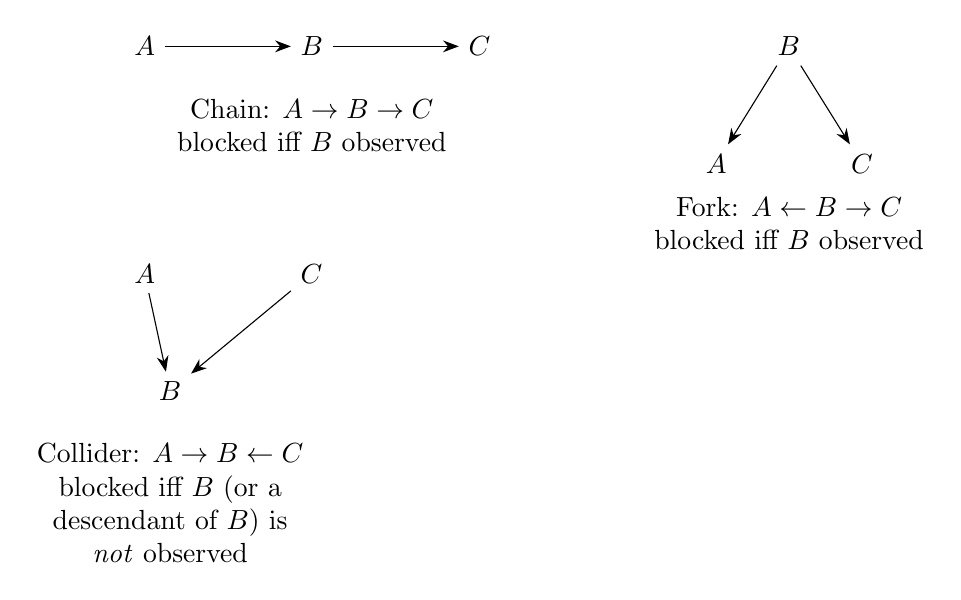
\begin{tikzpicture}[node distance=1.1cm and 1.6cm, >={Stealth[length=2mm]}]
  % Chain
  \node (A1) {$A$};
  \node[right=of A1] (B1) {$B$};
  \node[right=of B1] (C1) {$C$};
  \draw[->] (A1) -- (B1);
  \draw[->] (B1) -- (C1);
  \node[below=0.3cm of B1, align=center] {Chain: $A\to B\to C$\\blocked iff $B$ observed};

  % Fork
  \node[right=3.4cm of C1] (B2) {$B$};
  \node[below left=1.0cm and 0.4cm of B2] (A2) {$A$};
  \node[below right=1.0cm and 0.4cm of B2] (C2) {$C$};
  \draw[->] (B2) -- (A2);
  \draw[->] (B2) -- (C2);
  \node[below=0.3cm of $(A2)!0.5!(C2)$, align=center] {Fork: $A\leftarrow B\to C$\\blocked iff $B$ observed};

  % Collider
  \node[below=2.4cm of A1] (A3) {$A$};
  \node[right=1.6cm of A3] (C3) {$C$};
  \node[below right=1.0cm and -0.2cm of A3] (B3) {$B$};
  \draw[->] (A3) -- (B3);
  \draw[->] (C3) -- (B3);
  \node[below=0.3cm of B3, align=center] {Collider: $A\to B\leftarrow C$\\blocked iff $B$ (or a\\descendant of $B$) is\\ \emph{not} observed};
\end{tikzpicture}
\end{center}

\textbf{How to use this for $A \perp C \mid Z$:} enumerate every
undirected path between $A$ and $C$ in the graph. If \emph{every} path
is blocked according to the rules above (given the observed set $Z$),
then $A$ and $C$ are independent given $Z$. If even one path is
unblocked, they are (in general) \emph{not} independent given $Z$.
Two things people forget:
\begin{itemize}
  \item A chain or fork is blocked \emph{only if the middle node is in
        $Z$}; a collider is blocked \emph{only if the middle node
        (and none of its descendants) is in $Z$} --- this is the
        opposite condition, which is exactly why colliders create the
        ``explaining away'' effect (Problem 4, item 3 vs.\ item 4 is
        testing precisely this asymmetry).
  \item You must check \emph{all} paths, not just the shortest or most
        obvious one.
\end{itemize}

\section*{Problems 4(b), 5(b)-(c): Computing Marginals/Conditionals from a Factorized Joint}

Once you have the joint as a product of CPTs (from the graph structure),
any marginal or conditional you want is computed by two mechanical
steps:

\begin{enumerate}
  \item \textbf{Marginalize (sum out) variables you don't want}, e.g.
        \[
          p(d) = \sum_{a,t,s,l,b,e,x} p(a,t,s,l,b,e,x,d).
        \]
        Substitute the chain-rule factorization for the joint, then push
        each sum as far right as it will go (sum over a variable only
        after every factor involving it has been multiplied in) ---
        this is the idea behind \emph{variable elimination}, and it's
        far less error-prone than expanding the full $2^8$-row table by
        hand.
  \item \textbf{Condition by restricting and renormalizing}, e.g.\ for
        $p(d \mid s = \text{tr})$: fix $s=\text{tr}$ everywhere in the
        joint, sum out everything except $d$, and you already have an
        unnormalized version of $p(d, s=\text{tr})$; since
        $p(d\mid s=\text{tr}) = p(d,s=\text{tr})/p(s=\text{tr})$, either
        divide by $p(s=\text{tr})$ explicitly, or just normalize your
        two unnormalized values ($d=\text{tr}$ and $d=\text{fa}$) so
        they sum to 1 --- both give the same answer.
\end{enumerate}
For Problem 5(b)-(c), do the same thing symbolically instead of
numerically: write $p(x\mid z) = p(x,z)/p(z)$, expand $p(x,z)$ by
summing the full joint $p(x,y,w,z)$ over the variables not appearing
($y$ and $w$), and simplify using the given factorization
$p(x,y,w,z)=p(z\mid w)p(w\mid x,y)p(x)p(y)$.

\section*{Problem 5(d): Turning ``Equal Formulas'' into an Independence Condition}

$x \perp y \mid z$ means, by definition,
$p(x\mid y,z) = p(x\mid z)$ (equivalently $p(x,y\mid z)=p(x\mid z)p(y\mid z)$).
Using Bayes' rule (Problem 1's identity!) you can also write
$p(x\mid y,z) = \dfrac{p(y\mid x,z)\,p(x\mid z)}{p(y\mid z)}$. Comparing
this to the definition, $x\perp y\mid z$ holds exactly when
$p(y\mid x,z) = p(y\mid z)$ --- i.e.\ knowing $x$ (in addition to $z$)
doesn't change the distribution of $y$. Use your answers to parts (b)
and (c) (formulas for $p(x\mid z)$ and $p(y\mid z)$ in terms of the
given CPTs) to check whether this equality is forced by the given
factorization, or only holds under some extra condition --- state
which.

\section*{Practical tips}
\begin{itemize}
  \item For Problem 4(b), you're explicitly allowed to write code
        instead of hand-computing 8-variable sums. A skeleton notebook
        for this is provided separately
        (\texttt{chest\_clinic\_skeleton.ipynb}) --- fill in the CPTs
        from the table in the assignment and use nested loops /
        \texttt{itertools.product} to enumerate all variable
        assignments.
  \item Double check every CPT you write sums to 1 over the child
        variable for each fixed parent configuration --- this is the
        single most common source of arithmetic errors on these
        problems.
  \item For graph problems (3c, 4a, 5a, 6a-b), draw the graph and
        physically trace each path with your finger while checking the
        chain/fork/collider rule --- don't try to do it purely
        symbolically in your head.
\end{itemize}

\end{document}
